\documentclass{exam}

\usepackage{Haust2016verkefnablöð}

\title{Stærðfræðimynstur í tölvunarfræði \\ Skilaverkefni 12}
\author{}

\printanswers

\begin{document}
\maketitle
\thispagestyle{empty} 

Skila skal þessu verkefni á vefnum \href{https://gradescope.com/}{Gradescope}. Aðgangskóði fyrir námskeiðið er \textbf{926WD9}. Allar heiðarlegar tilraunir til að leysa þetta verkefni gefa einkunnina 10.

\section{Spurningar}

\begin{questions}

\section{Kafli 11.4}

\question Notið dýptarleit til að finna spanntré fyrir eftirfarandi net. Veljið $a$ sem rót. Þegar velja þarf á milli jafngildra hnúta, veljið í stafrófsröð. Gefið lausn með því að telja leggina upp í röð.

\begin{center}
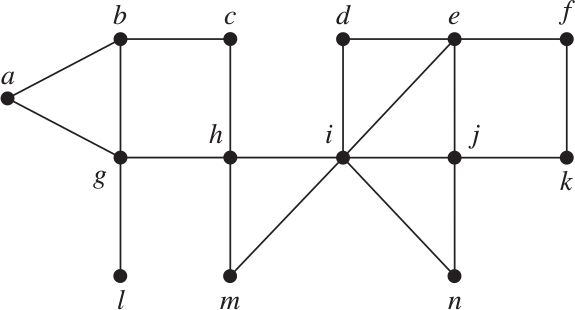
\includegraphics[width=0.5\textwidth]{tree-spanning-exercise}
\end{center}

\paragraph{Í bók:} Exercise 11.4.14

\section{Kafli 11.5}

\question Finnið tvö léttustu spanntré í eftirfarandi neti, annars vegar með reikniriti Prims og hins vegar með reikniriti Kruskals. Gefið lausn með því að telja leggina upp í röð.

\begin{center}
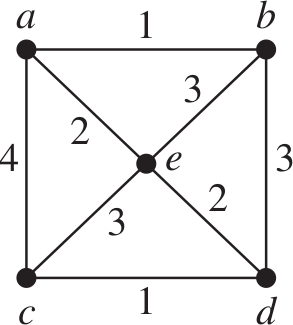
\includegraphics[width=0.2\textwidth]{tree-spanning-minimum-exercise}
\end{center}

\paragraph{Í bók:} Byggt á Exercise 11.5.2

\section{Kafli 13.2}

\question Skrifið endanlega stöðuvél sem hefur bitastreng sem inntak og bitastreng sem úttak. Úttaksstrengurinn skal hefjast á $00$ en annars vera eins og inntaksstrengurinn seinkaður um tvo bita.

Gefið lausn með því að teikna stöðuvélina.

\paragraph{Í bók:} Exercise 13.2.9

\question Skrifið endanlega stöðuvél sem hefur bitastreng sem inntak og bitastreng sem úttak. Úttaksstrengurinn skal hafa $1$ ef fjöldi bita sem lesinn hefur verið inn er deilanlegur með 3, en $0$ annars.

Gefið lausn með því að teikna stöðuvélina.

\paragraph{Í bók:} Exercise 13.2.16

\section{Kafli 13.3}

\question Lýsið mengi strengjanna sem eftirfarandi stöðuvél samþykkir.

\begin{center}
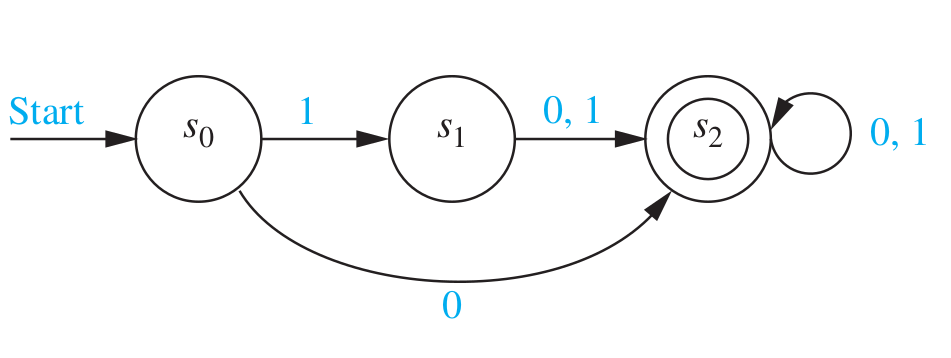
\includegraphics[width=0.5\textwidth]{dfa-exercise}
\end{center}

\paragraph{Í bók:} Exercise 13.3.17

\question Skrifið endanlega stöðuvél sem samþykkir (eingöngu) mengi þeirra bitastrengja sem samanstanda af $0$ og svo oddatölufjölda $1$.

Gefið lausn með því að teikna stöðuvélina.

\paragraph{Í bók:} Exercise 13.3.35

\end{questions}

\end{document}